\chapter{Strumento di Versioning}

\section{Scelte adottate}
GitHub è una piattaforma di hosting per il controllo di versione e la collaborazione, costruita attorno al sistema di versioning distribuito Git. Questo strumento è ampiamente utilizzato nella comunità degli sviluppatori per gestire progetti software.
\\
Per il versioning di \textbf{DietiDeals24} abbiamo scelto proprio Github, andando a separare la repository del Client, da quella del Server, per una maggiore organizzazzione del progetto. 

\subsection{Vantaggi di GitHub come strumento di versioning}

L'utilizzo di GitHub come strumento di versioning presenta numerosi vantaggi, tra cui:

\subsubsection*{1. Collaborazione facilitata}
GitHub consente a più sviluppatori di lavorare contemporaneamente sullo stesso progetto senza conflitti. Attraverso le funzionalità di pull request, gli utenti possono proporre modifiche al codice, che possono essere revisionate e integrate nel progetto principale. Questo processo rende la collaborazione più fluida e organizzata.

\subsubsection*{2. Tracciamento delle modifiche}
Ogni modifica apportata al codice è registrata nella cronologia del repository. Gli sviluppatori possono visualizzare chi ha apportato una modifica, quando e perché, il che aiuta a mantenere una documentazione chiara delle evoluzioni del progetto.

\subsubsection*{3. Ritorno a versioni precedenti}
GitHub consente di annullare modifiche o di tornare a versioni precedenti del codice. Questo è particolarmente utile quando una nuova funzionalità introduce un bug o quando è necessario ripristinare un comportamento precedente.

\subsubsection*{4. Backup e sicurezza}
I repository su GitHub sono ospitati nel cloud, fornendo un backup sicuro del codice.

\section{Repository Client}
\url{https://github.com/progetto-INGSW-23-24/flutter-app}
\sskip
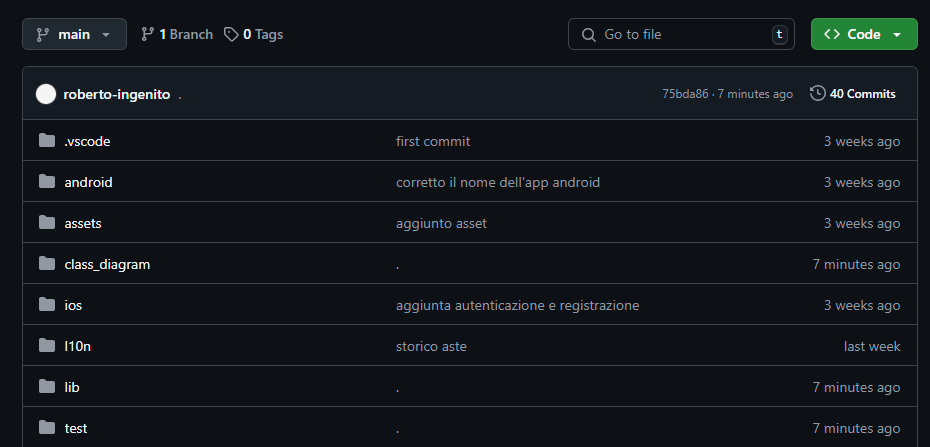
\includegraphics[width=\textwidth]{assets/versioning_screens/client.png}

\section{Repository Server}
\url{https://github.com/progetto-INGSW-23-24/backend}
\sskip
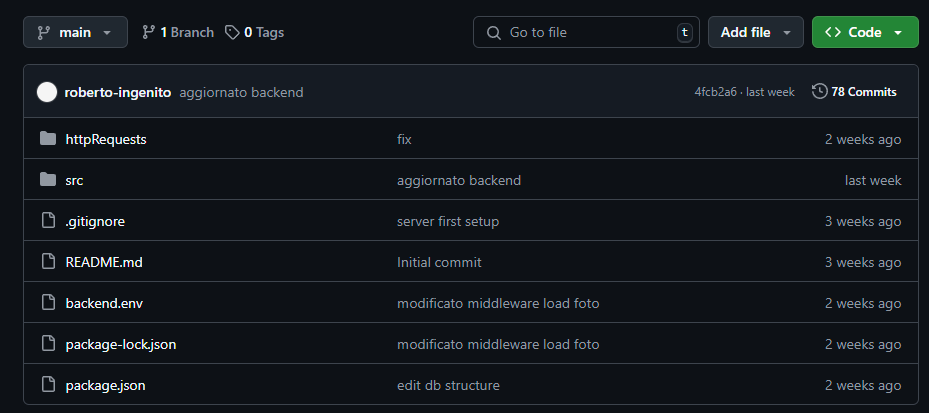
\includegraphics[width=\textwidth]{assets/versioning_screens/server.png}

